% !TeX root = ../Main-Report.tex

\chapter{Joint Space Motion}

In this section, the process of oding joint space motions with the robot is documented. First, three waypoints are chosen inside of the workspace of the robot. They can be seen in table \ref{tab:jspace_waypoints}.

\begin{table}[H]
\centering
\caption{Chosen waypoints for trajectory planning}
\label{tab:jspace_waypoints}
\begin{tabular}{llll}
	Waypoint & $x$    & $y$    & $z$   \\ \hline
	$1$      & $0.0$  & $0.0$  & $0.4$ \\
	$2$      & $0.1$  & $0.1$  & $0.4$ \\
	$3$      & $-0.1$ & $-0.1$ & $0.4$ \\
	$4$      & $0.1$  & $-0.1$ & $0.4$ \\
	$5$      & $0.0$  & $0.0$  & $0.0$
\end{tabular}
\end{table}

Using the acceleration and velocity constraints that were given in the task, the synchronized velocity profile has been calculated in the file \textit{jspace\_trapz.m}. The outputs are time stamps and corresponding velocity values, which are then input into a Repeating table block in Simulink and fed into an integrator to receive the needed position information. As the simulation uses the vectors from the workspace, the script \textit{jspace\_trapz.m} needs to be run before the simulation.

\begin{figure}[H]
	\centering
	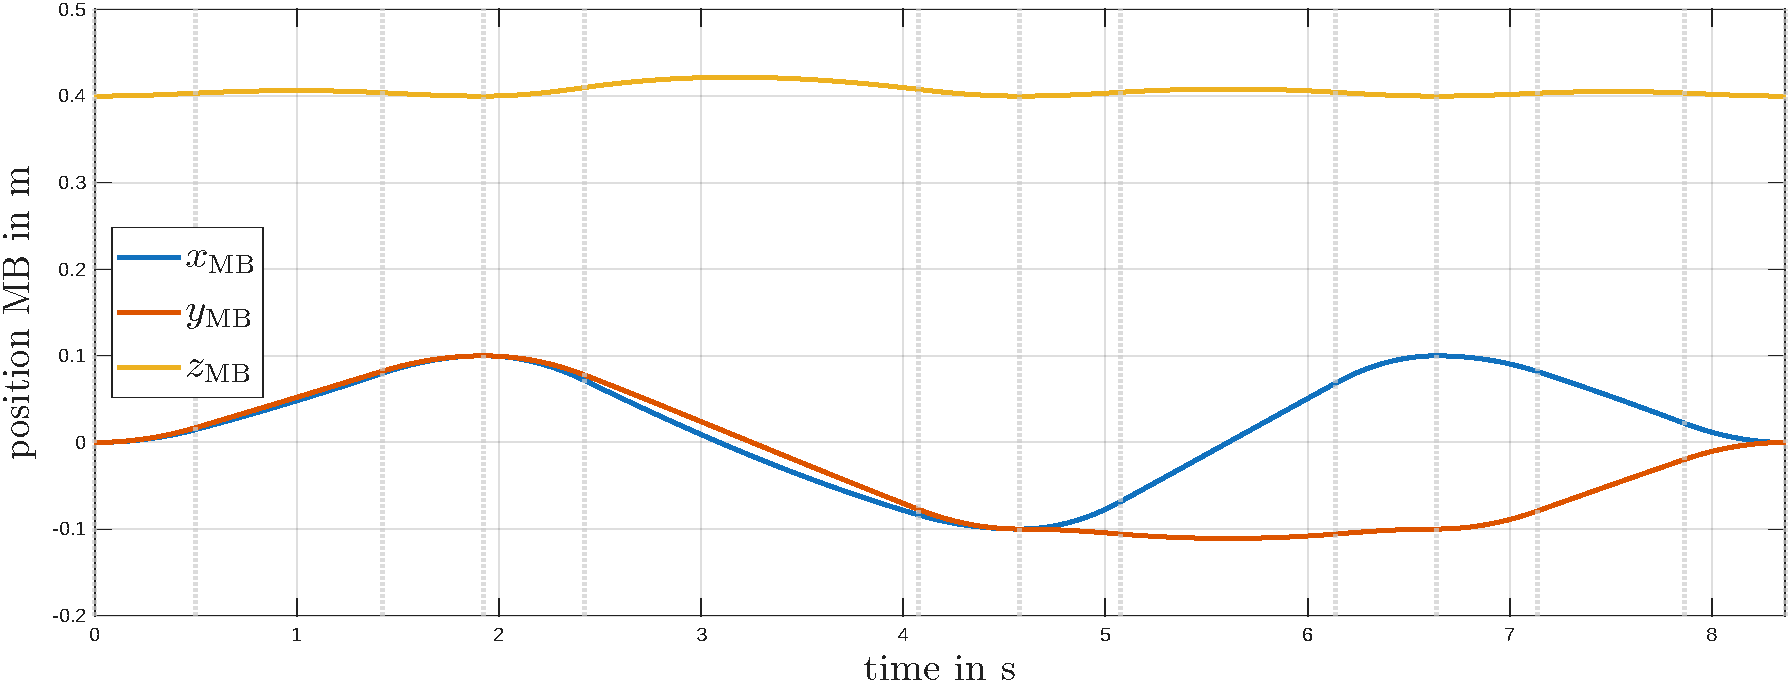
\includegraphics[width=1.0\linewidth]{cus_imgs/joint_trapz_xyz.pdf}
	\caption{$x$, $y$ and $z$ position of the end-effector for the trapezoidal velocity profile}
	\label{fig:jspace_trapz_xyz}
\end{figure}

Figure \ref{fig:jspace_trapz_xyz} shows the position of the end-effector of the robot when following the trapezoidal trajectory. The trajectory itself, with position, velocity and acceleration profile can be viewed in figure \ref{fig:jspace_trapz_traj}.

\begin{figure}[H]
	\centering
	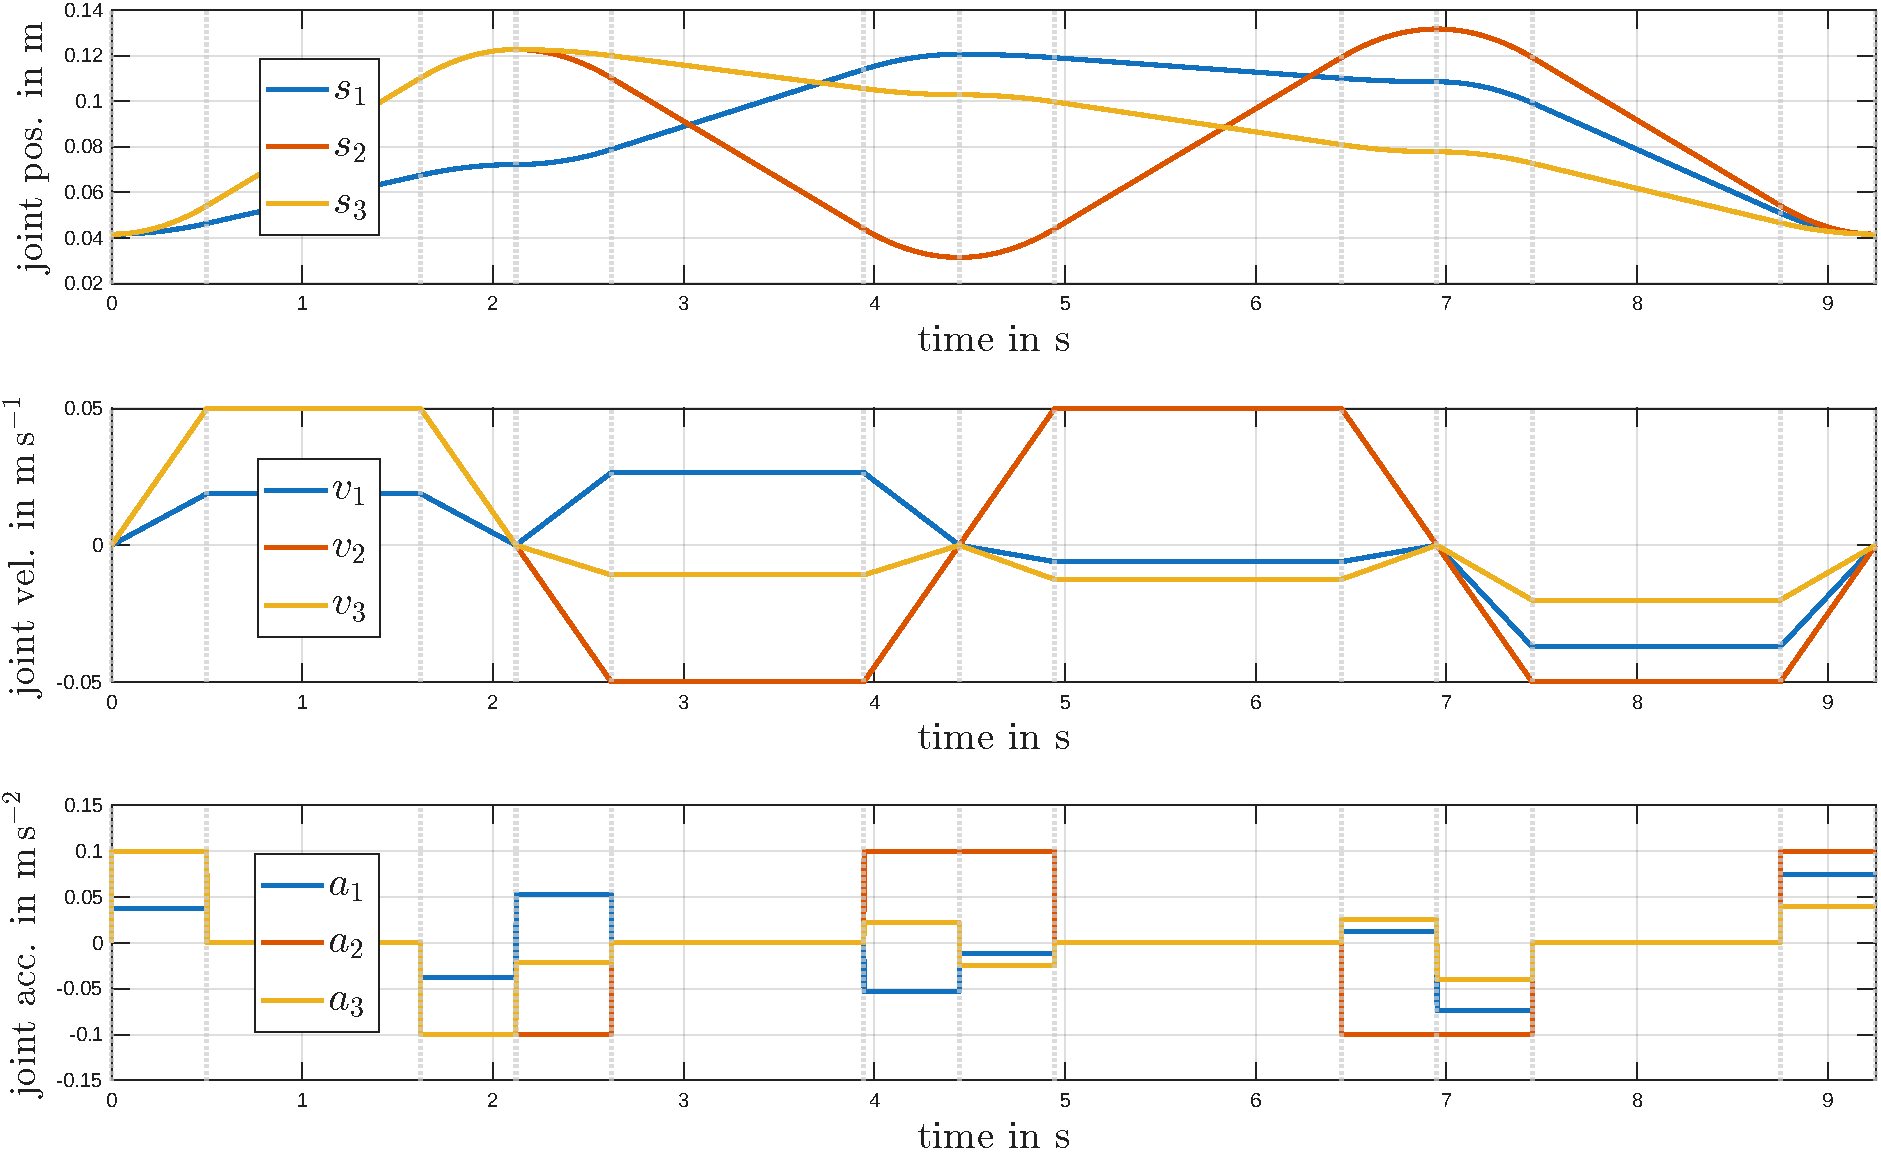
\includegraphics[width=1.0\linewidth]{cus_imgs/joint_trapz.pdf}
	\caption{Generated trajectory, including position, velocity and acceleration profiles}
	\label{fig:jspace_trapz_traj}
\end{figure}